\chapter{Systemarkitektur (Alle)}

\section{Version}
\begin{table}[h]
	\centering
	\begin{tabularx}{\textwidth - 2cm}{|l|l| l|X|}
	\hline
	Dato	& Version	& Initialer & Ændring	\\ \hline
	29. oktober & 1 & LS	& Første udkast af dokumentet. \\ \hline
	19. november & 2 & KT & Mange mindre rettelser efter review. \\ \hline
	02. december & 3 & HBJ & Rettelser af lampe signaler. \\ \hline
	15. december & 4 & LS & Mindre rettelser. Endelig version. \\ \hline
	\end{tabularx}
\end{table}

\section{SysML diagrammer}
Beskrivelse af samtlige signaler findes i Tabel \ref{tbl:signalbeskriv} på side \pageref{tbl:signalbeskriv}.

\subsection{BDD for system kontekst}

I Figur \ref{fig:bddcontext} vises konteksten for systemet, som består af de elektriske enheder samt brugeren af systemet. Yderligere vises porte på aktørerne, som agerer med systemet. Bruger blokken beskriver den person der interagerer med systemet. Radio blokken er en radio med mulighed for styring via en IR fjernbetjening, TV blokken er tilsvarende. De to lampe blokke er to $5V$ lyskilder, som kan dimmes via pulsbreddemodulation.

Bemærk at ingen blokke eller enheder forsynes fra $18 VAC$ nettet, da dette kun bruges til X.10 kommunikation. Der benyttes derimod eksterne spændingsforsyninger.

\begin{figure}[h]
	\centering \resizebox{\textwidth}{!}{
	\includegraphics[scale=1,trim=17 310 300 15, clip=true]{Systemarkitektur/Diagrammer/BDD_System_Context}}
	\caption{BDD for system konteksten}
	\label{fig:bddcontext}
\end{figure}

\clearpage

\subsection{IBD for system kontekst}
I Figur \ref{fig:IBDsystemContext} vises systemets eksterne forbindelser til de øvrige blokke omkring systemet.

\begin{figure}[h]
	\centering \resizebox{\textwidth}{!}{
	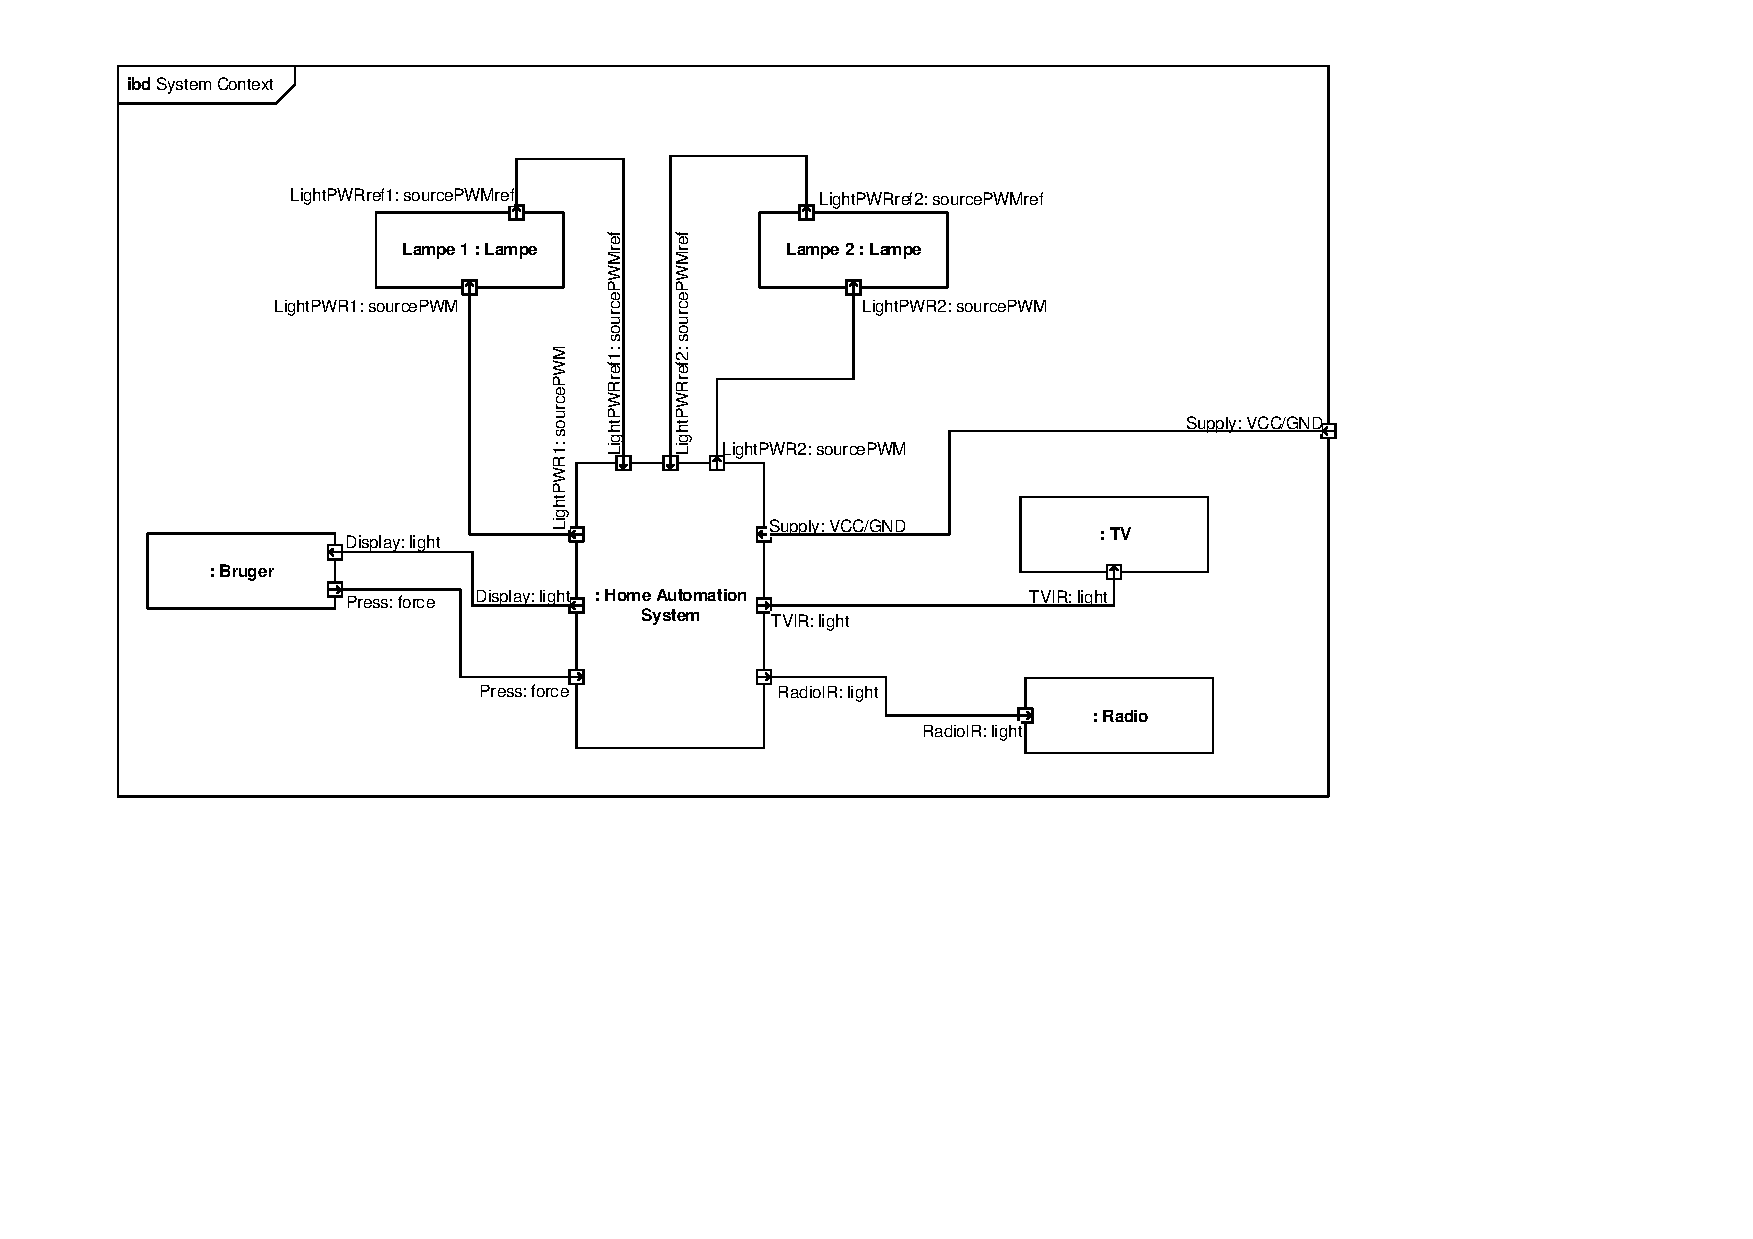
\includegraphics[width={\textwidth}, trim=55 200 200 15, clip=true]{Systemarkitektur/Diagrammer/IBD_System_Context.pdf}}
	\caption{IBD for system konteksten}
	\label{fig:IBDsystemContext}
\end{figure}

Det antages at der til TV samt Radio allerede er tilført spændingsforsyninger, da disse enheder ikke er en del af systemet.

\clearpage

\subsection{BDD for systemet}

I Figur \ref{fig:BDDsystem} vises et BDD over systemet i sin helhed. Diagrammet viser overordnede blokke i systemet, samt deres ports og parts.

PC blokken er brugerens grænseflade til systemet. Transmitterblokken modtager information fra PC softwaren, såfremt kodelåsen er aktiveret, og sender kommandoer til Receiver-blokkene.

Receiver-blokkene består kun af receivere, dvs. selve TV'et, Radioen og lamperne ikke er en del af systemet.

Der er for overskuelighedens skyld valgt ikke at indskrive systemets porte i <<System of interest>> blokken. Disse fremgår af Figur \ref{fig:IBDsystemContext}.


\begin{figure}[h]
	\centering \resizebox{\textwidth}{!}{
	\includegraphics[scale=1,trim=28 210 219 25, clip=true]{Systemarkitektur/Diagrammer/BDD_system}}
	\caption{BDD diagram for systemet}
	\label{fig:BDDsystem}
\end{figure}

\clearpage

\begin{landscape}

\subsection{IBD for systemet}

I Figur \ref{fig:IBDsystem} vises de interne forbindelser mellem blokke i systemet. Selve lampen får sin forsyning gennem \emph{LightPWR: SourcePWM} og har en referance fra \emph{LightPWRref: SourcePWMref}. Signaltypen \emph{signal} har sin reference via \emph{VCC/GND}.

\begin{figure}[h]
	\centering \resizebox{!}{\textwidth -3.5 cm}{
	\includegraphics[scale=1,trim=30 170 158 45, clip=true]{Systemarkitektur/Diagrammer/IBD_Home_Automation_system.pdf}}
	\caption{IBD diagram for Home Automation systemet}
	\label{fig:IBDsystem}
\end{figure}

\end{landscape}

\clearpage

\subsection{IBD for Transmitter-blokken}

I Figur \ref{fig:IBDtransmitter} vises de interne forbindelser mellem parts i Transmitter-blokken.

\begin{figure}[h]
	\centering
	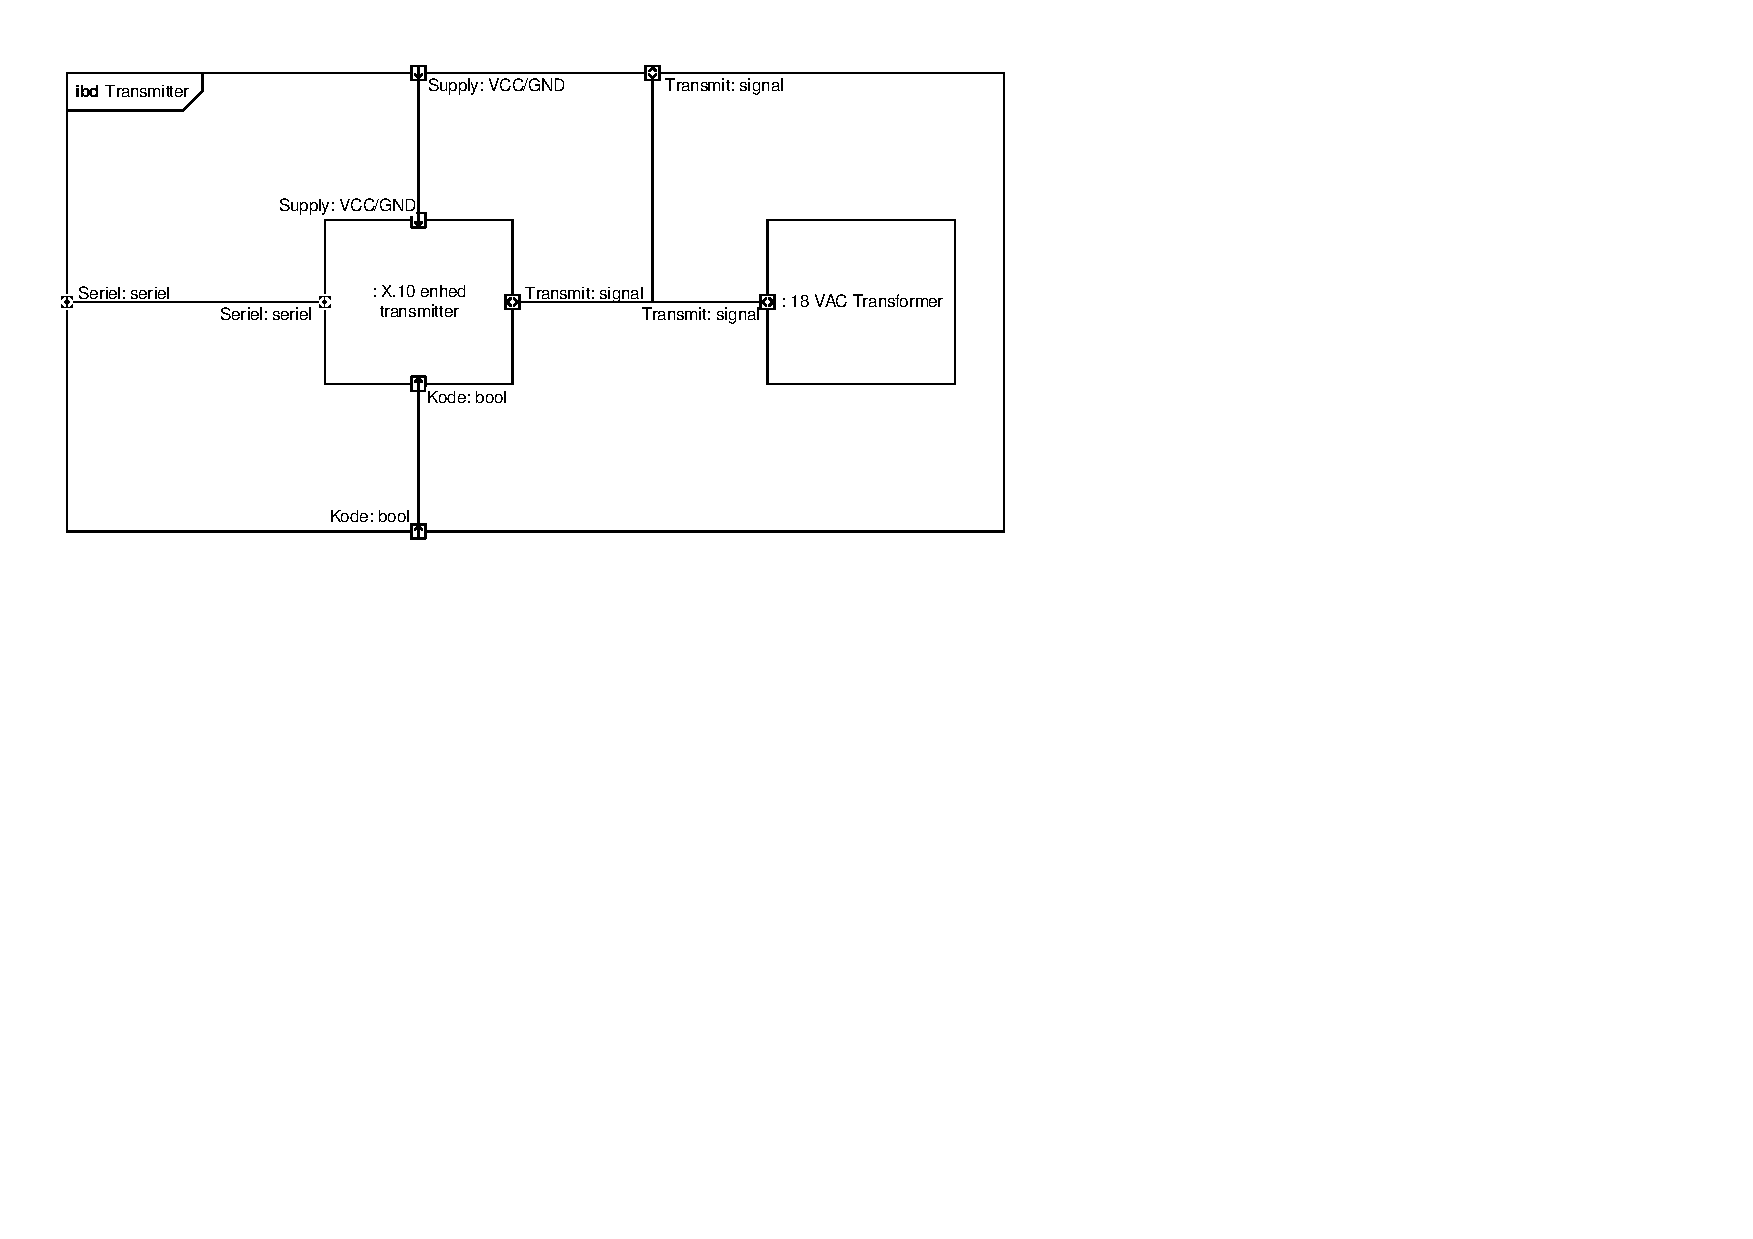
\includegraphics[scale=1,trim=30 335 350 30, clip=true]{Systemarkitektur/Diagrammer/IBD_Transmitter.pdf}
	\caption{IBD for Transmitter}
	\label{fig:IBDtransmitter}
\end{figure}

\subsection{IBD for X.10-enhed i transmitter-blokken}

I Figur \ref{fig:IBDx.10transmit} vises forbindelser mellem STK500 og øvrig hardware i blokken, og dermed grænsefladen mellem software og hardware.

\begin{figure}[h]
	\centering \resizebox{\textwidth}{!}{
	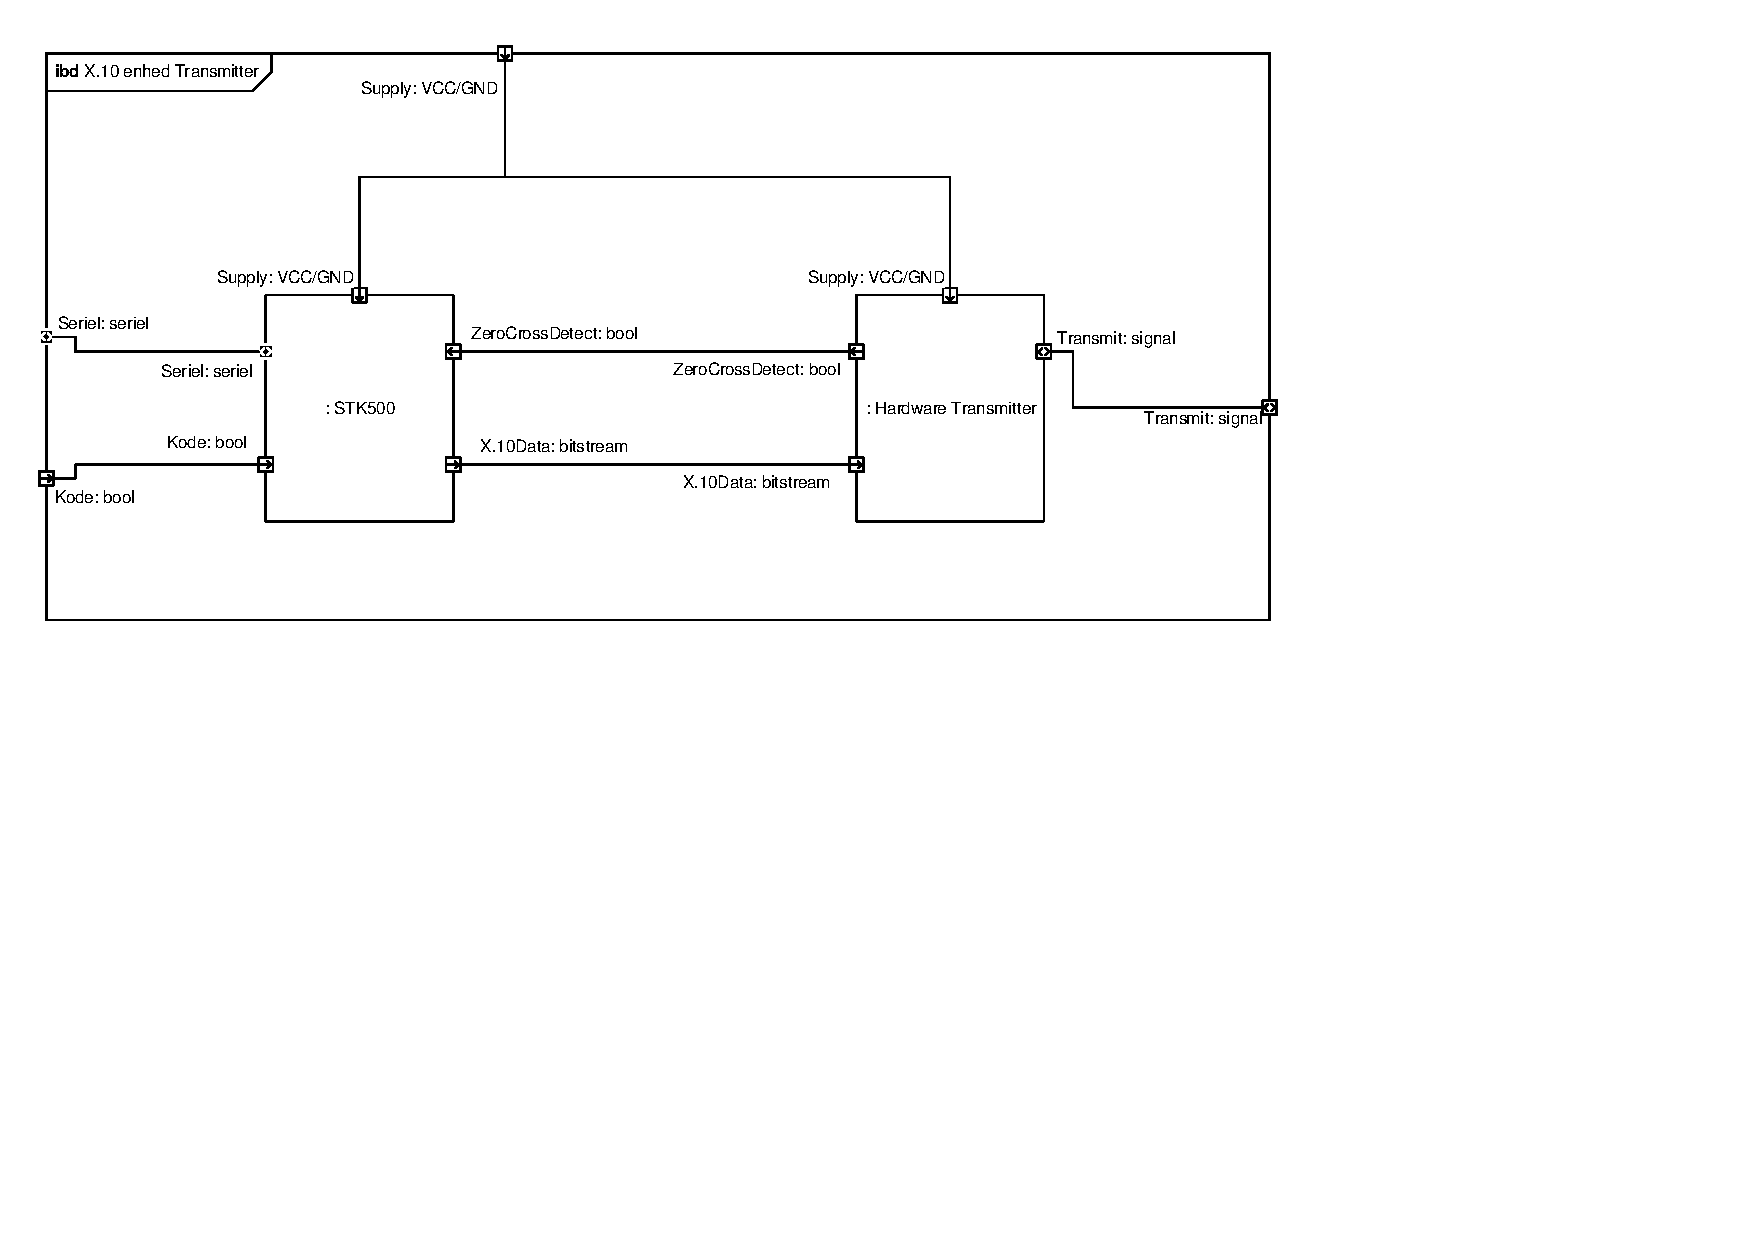
\includegraphics[scale=1,trim=18 295 220 20, clip=true]{Systemarkitektur/Diagrammer/IBD_X10_Enhed_Transmitter.pdf}}
	\caption{IBD for X.10 enheden i transmitteren}
	\label{fig:IBDx.10transmit}
\end{figure}

\clearpage

\begin{landscape}
\subsection{IBD for receivers}

I Figur \ref{fig:IDBreceivers} vises samtlige typer af receivers i systemet. Af hensyn til overskuelighed vises der kun én instans af Receiver Lys, selvom systemet reelt indeholder to, jf multiplicitet i Figur \ref{fig:BDDsystem} side \pageref{fig:BDDsystem}.

\begin{figure}[h]
	\centering \resizebox{!}{\textwidth - 4 cm}{
	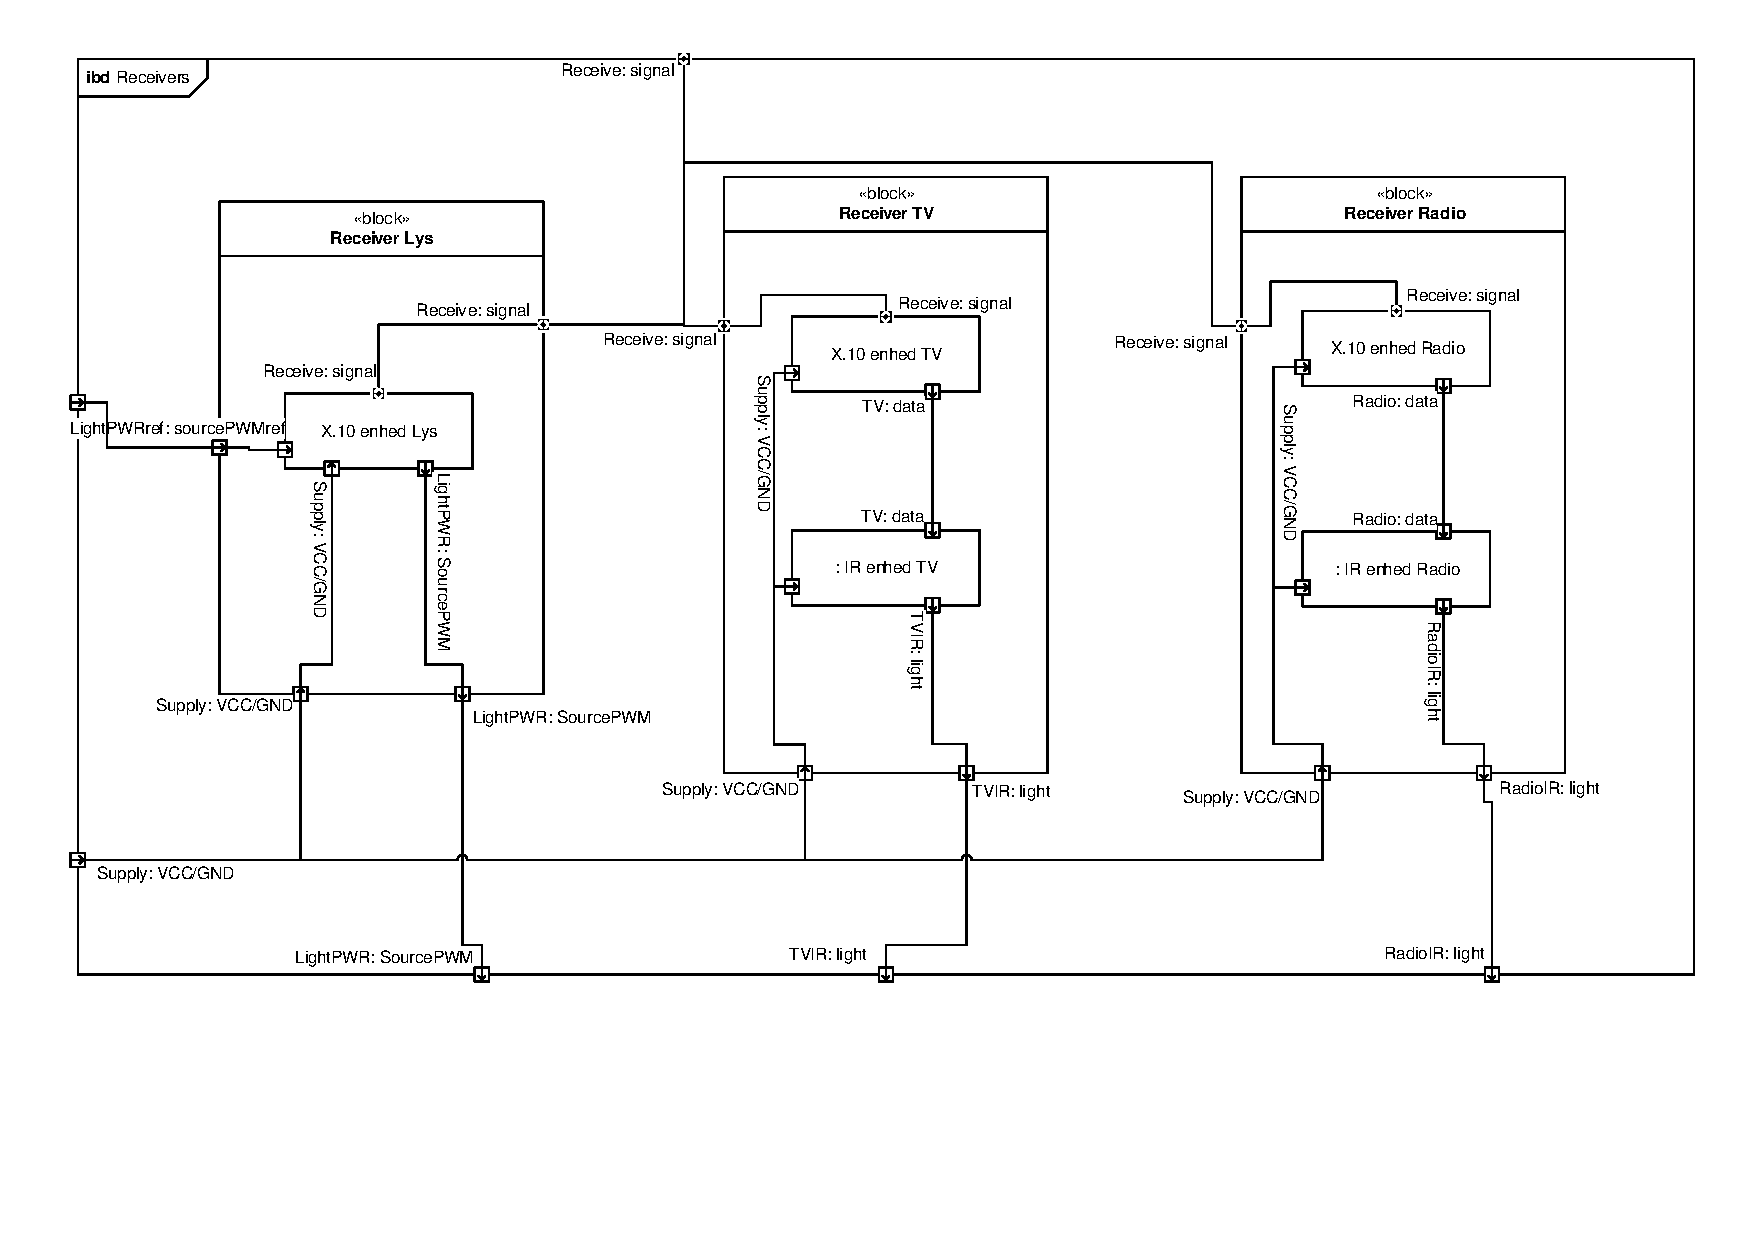
\includegraphics[scale=1,trim=30 122 10 25, clip=true]{Systemarkitektur/Diagrammer/IBD_Receivers.pdf}}
	\caption{IBD for receivers}
	\label{fig:IDBreceivers}
\end{figure}
\end{landscape}

\clearpage
\begin{landscape}
\subsection{IBD for X.10 enhed i lys-blokken} \label{subsec:IBDX10Lys}

I Figur \ref{fig:IDBx.10lys} vises forbindelser mellem STK500 og øvrig hardware i blokken, og dermed grænsefladen mellem software og hardware.

\begin{figure}[h]
	\centering \resizebox{\textwidth}{!}{
	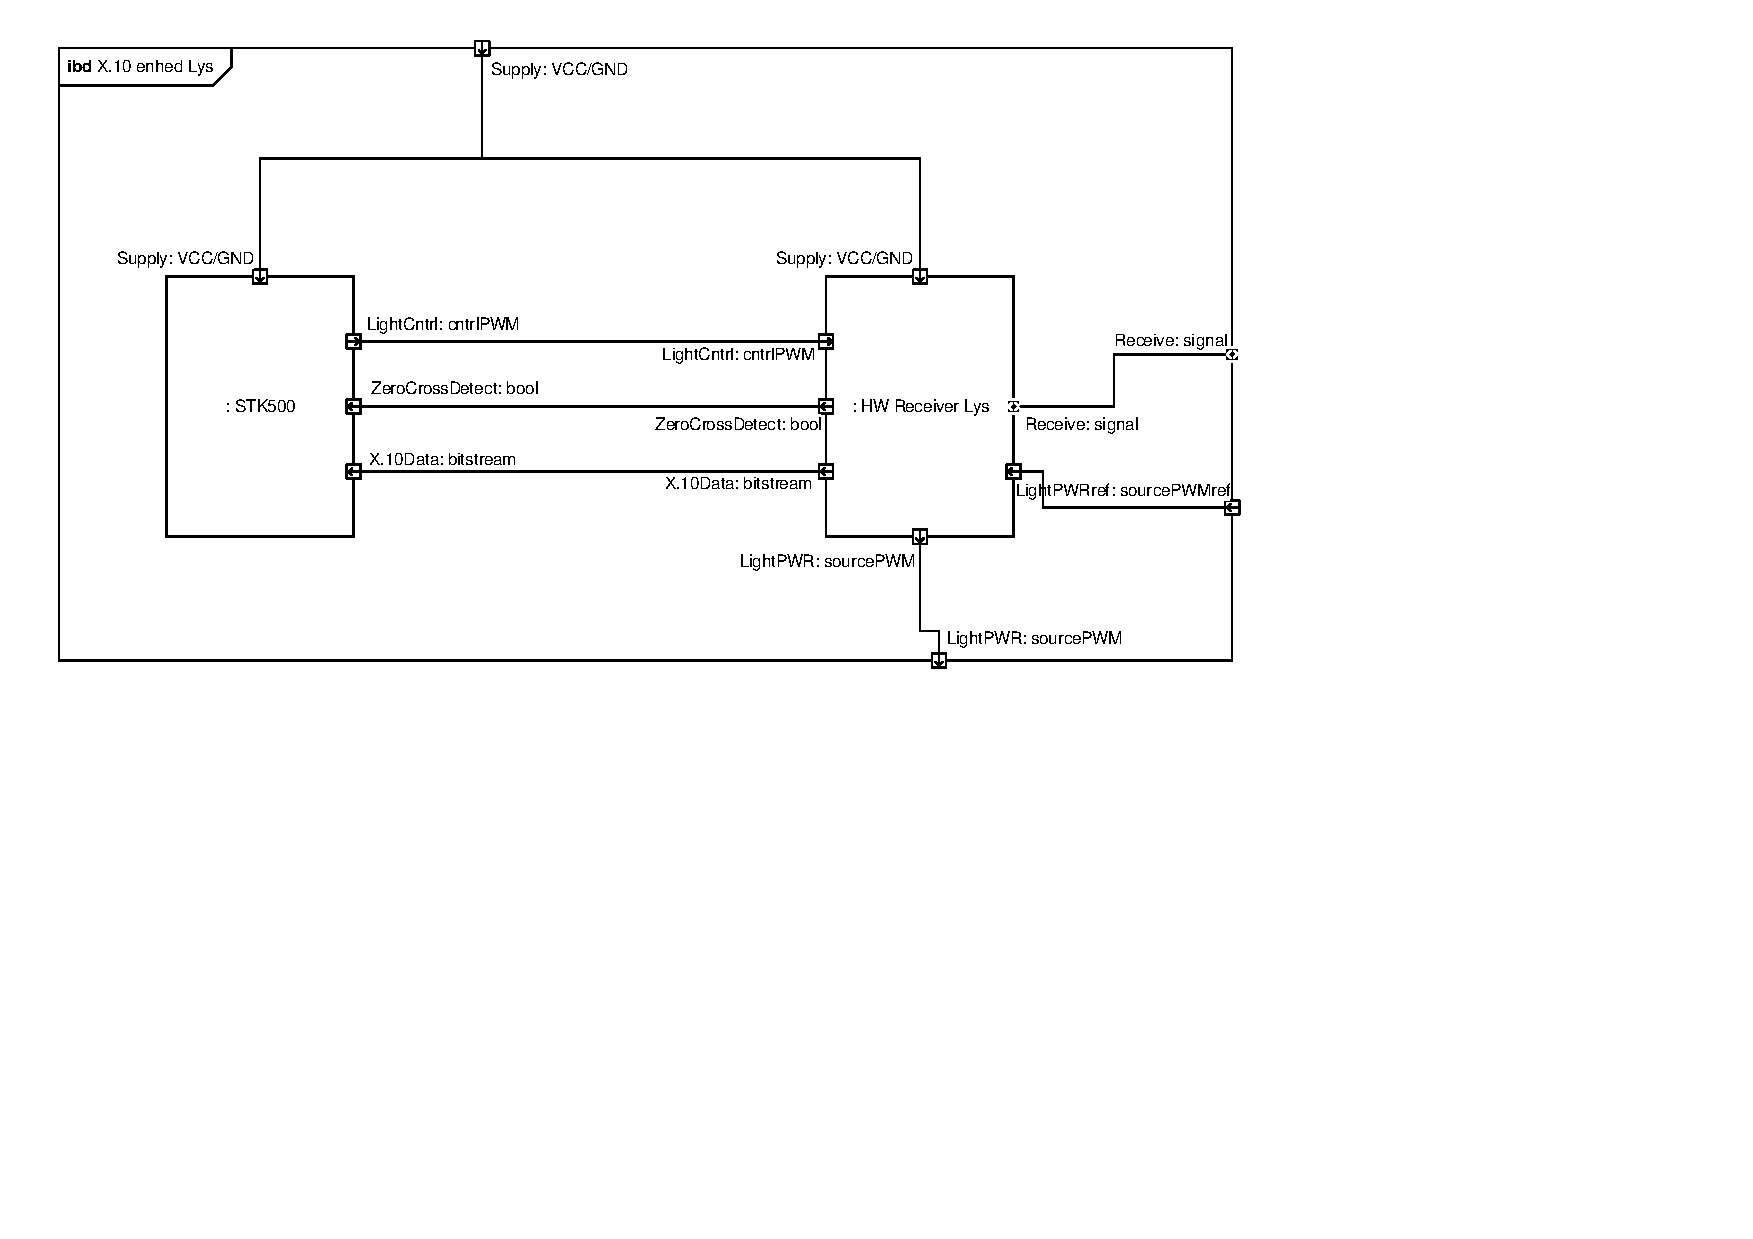
\includegraphics[height={\textwidth+5cm},trim=25 270 245 20, clip=true]{Systemarkitektur/Diagrammer/IBD_X10_Enhed_Receiver_Light.pdf}}
	\caption{IBD for X.10 enheden i transmitteren}
	\label{fig:IDBx.10lys}
\end{figure}
\textbf{NOTE:}
Bemærk at projektdokumentationen indtil dette punkt har indeholdt det komplette system, men fra dette punkt behandles TV- og Radio-delen af systemet ikke. Dvs. at en del af signalerne ikke er beskrevet samt at videre dokumentationer og design ikke omfatter TV- og Radio-delen.
\end{landscape}


\clearpage
\section{Signalbeskrivelser}
\subsection{Signaltyper}
Grænseværdierne for samtlige signaler, som har kontakt med STK500 er defineret ud fra tolerencerne på ATMega32's porte\cite{lib:AtMega32}.
\begin{table}[h]
\centering
\begin{tabularx}{\textwidth}{| l | >{\raggedright}X | >{\raggedright}X | >{\raggedright\arraybackslash}X |}
\hline
	Signaltype & Funktion & Område & Kommentar \\ \hline
	bitstream & Serie af 1'er og 0'er & HIGH: $3.1 - 5.4V$, LOW: $-0.4 - 0.9V$ & 1 = Tilstedeværelse af $120 kHz$ signal, som går fra LOW til HIGH. 0 = LOW \\ \hline
	cntrlPWM & Firkantformet PWM signal på 1 kHz til regulering af lysstyrke & $0.0 - 5.0 V$ maks $10 mA$.  & PWM duty cycle kan variere i området $5\%-95\%$ i trin af $10\% \pm 1\%$.  \\ \hline
	force & Brugerens input på PC & \  & \  \\ \hline
	light & Output på PC'ens skærm & \  & \  \\ \hline
	seriel & Kommunikation mellem PC og transmitter & jf. RS232 & \  \\ \hline
	signal & Sammensætning af $18V AC$  og X.10 & $18V AC \pm 10\%$ \cite{lib:Adaptor} & $18V AC$ leveres fra transformeren og X.10 ($120 kHz$ i nulgennemgange) leveres fra Transmitter-blokken.  \\ \hline
	sourcePWM & Firkantformet PWM spændingsforsyning på 1 kHz til at drive lys & $5.0V \pm 0.1V$ & \\ \hline	
	sourcePWMref & Reference til lampe & $0.0V - (2.9V \pm 0.5V)$ med samme frekvens som cntrlPWM & \\ \hline
	VCC/GND & DC spændingsforsyning og reference & VCC: $11.8 - 12.2V$, GND: $0.0V$ & Signalet er en sammensætning af to forbindelser, VCC og stel. \\ \hline
	bool & Kan være enten HIGH (1) eller LOW (0) & HIGH: $3.1 - 5.4V$, LOW: $-0.4 - 0.9V$ & 1 = HIGH, 0 = LOW \\ \hline
\end{tabularx}
\caption{Beskrivelse af samtlige signaler.}
\label{tbl:signalbeskriv}
\end{table}
\clearpage
\subsection{Grænseflader}

\begin{itemize}
\item \emph{ZeroCrossDetected: bool} \\
Skal toggle hver gang der registreres en nulgennemgang på \emph{Transmit: Signal}.

\item \emph{Receive: Signal} \& \emph{Transmit: Signal} \\
Består af et $18 VAC$ ved $50 Hz$, som for hver nulgennemgang til $1 ms$ efter kan indeholde $120 KHz$ signaler. Hvis der forefindes et $120 KHz$ signal i en nulgennemgang, betragtes det som HIGH. Hvis der ikke forefindes et $120 KHz$ signal, betragtes det som LOW.

\item \emph{X.10Data: bitstream} \\
Signalet er grænsefladen mellem STK500 og hhv. transmitter og receiver. HIGH på signalet svarer til at der forefindes $120 kHz$ på \emph{signal}. Når signalet bruges til at sende med skal det holdes HIGH i $1 ms$ fra nulgennemgang.

\item \emph{Kode: bool} \\
Er LOW hvis koden er indtastet korrekt og HIGH hvis den ikke er indtastet korrekt.

\item \emph{Seriel: seriel} \\
BAUD rate på 9600, 8 bit, 1 startbit, 2 stopbit og ingen paritet.

\item \emph{LightCntrl: CntrlPWM} \\
Firkantformet PWM styresignal til regulering af \emph{LightPWR: SourcePWM}.

\item \emph{LightPWR(1} \& \emph{2): SourcePWM} \\
Firkantformet PWM forsyningssignal til at drive lampen. Duty cycle samt frekvens for \emph{LightPWR: SourcePWM} og \emph{LightCntrl: CntrlPWM} skal være ens.

\item \emph{LightPWRref(1} \& \emph{2): SourcePWMref} \\
Reference til \emph{LightPWR: SourcePWM}. Samme frekvens og duty cycle som \emph{LightPWR: SourcePWM}.
\end{itemize}


\section{Softwarearkitektur}
For samtlige diagrammer gælder det at prækonditioner til de enkelte UC er medtaget.

\subsection{Sekvensdiagram for PC [Use Case 1: Opret Scenarie]}
Diagrammet i Figur \ref{fig:PC_UC1Sek} viser sekvenser for PC'en ved gennemgang af hovedscenariet i UC1. Når der oprettes et objekt af klassen Scenario, oprettes det automatisk med 20 tomme aktioner.

\begin{landscape}
\begin{figure}
	\centering %\resizebox{\textwidth}{!}{
	\includegraphics[height=\textwidth - 30 pt,trim=18 15 17 18, clip=true]{Systemarkitektur/Diagrammer/PC_UC1_Sekvens.pdf}%}
	\caption{Sekvensdiagram for PC [Use Case 1: Opret Scenarie]}
	\label{fig:PC_UC1Sek}
\end{figure} 

\end{landscape}

\clearpage

\subsection{Sekvensdiagram for PC [Use Case 2: Vælg Scenarie]}
Diagrammet viser sekvenser for PC'en ved gennemgang af hovedscenariet i UC2.
\begin{figure}[h]
	\centering %\resizebox{\textwidth}{!}{
	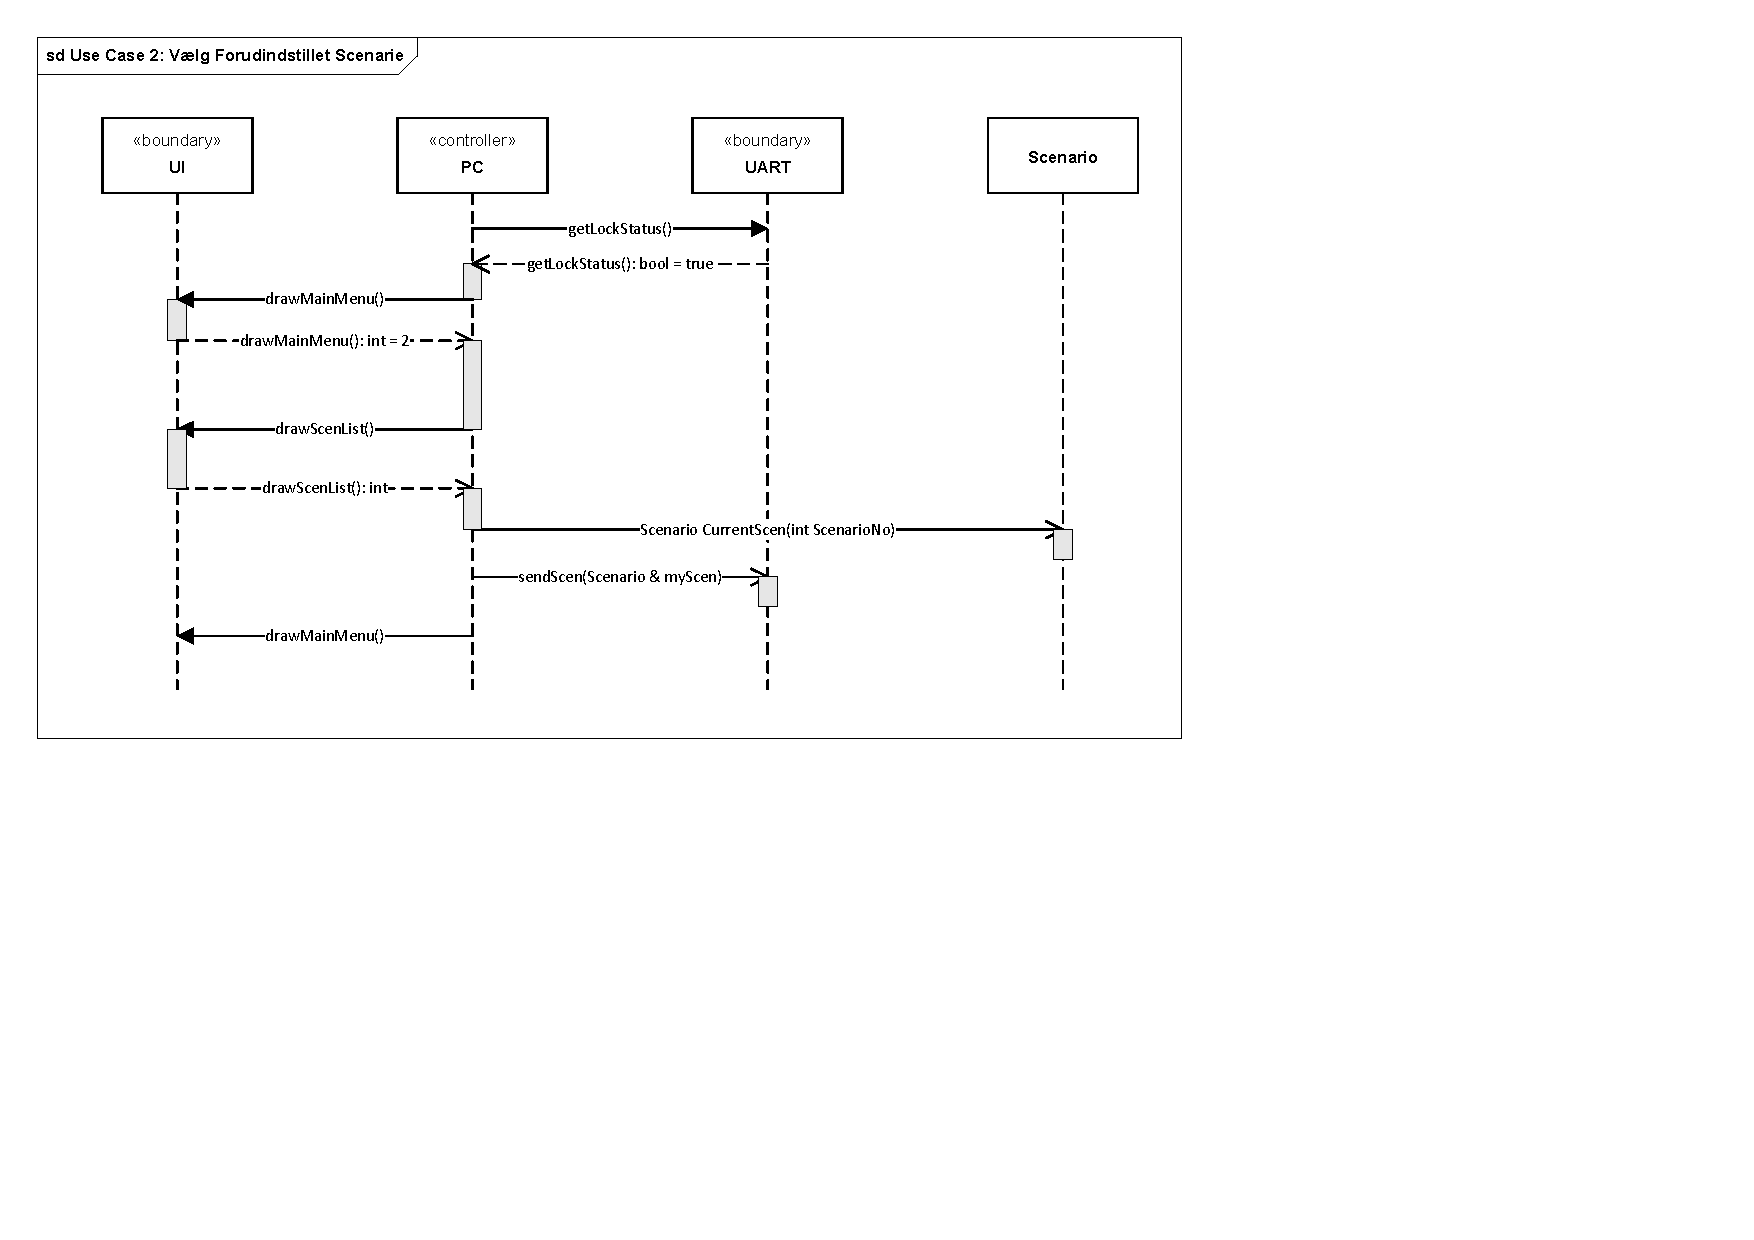
\includegraphics[width=\textwidth ,trim=17 235 274 18, clip=true]{Systemarkitektur/Diagrammer/PC_UC2_Sekvens.pdf}%}
	\caption{Sekvensdiagram for PC [Use Case 2: Vælg Scenarie]}
	\label{fig:PC_UC2Sek}
\end{figure}

\clearpage

\subsection{Sekvensdiagram for PC [Use Case 3: Stop Scenarie]}
Diagrammet viser sekvenser for PC'en ved gennemgang af hovedscenariet i UC3. 
\begin{figure}[h]
	\centering \resizebox{\textwidth}{!}{
	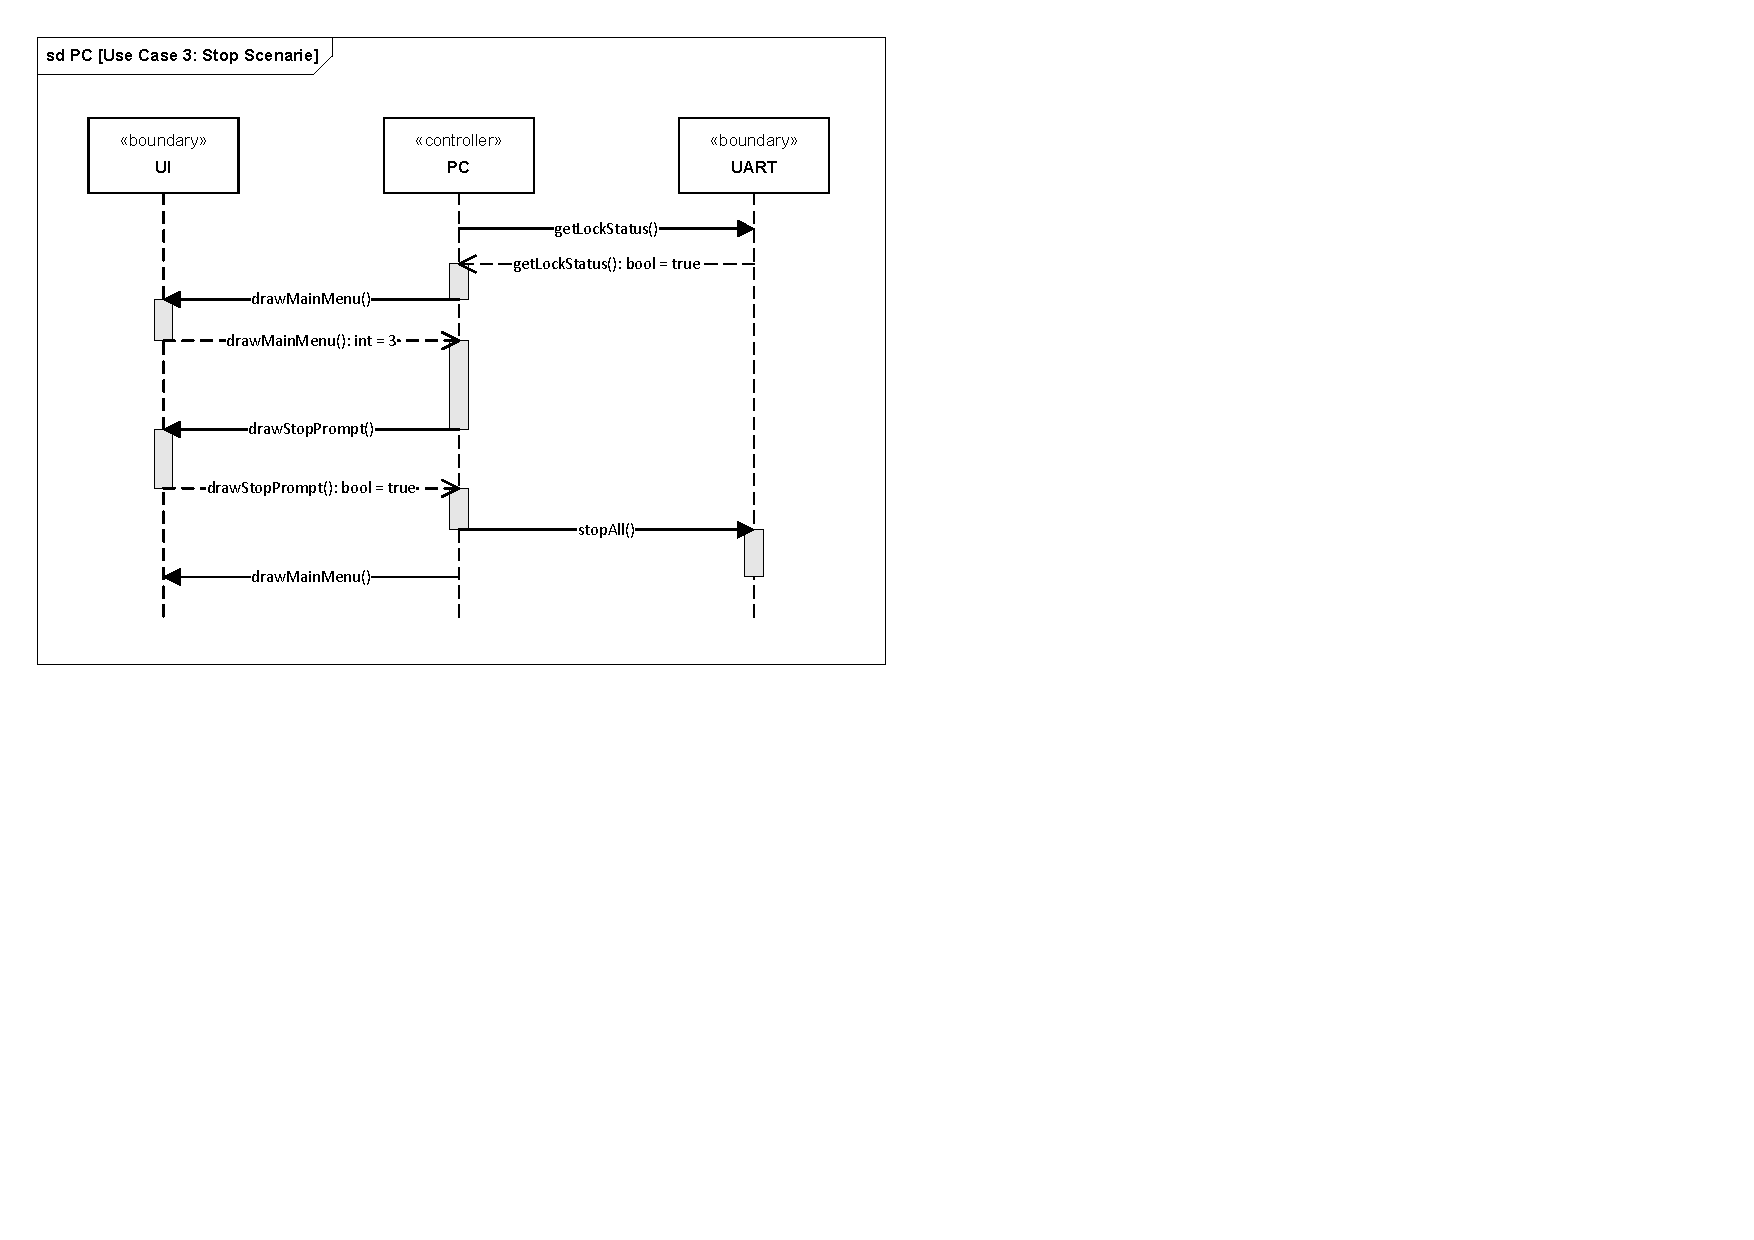
\includegraphics[scale=1,trim=18 270 400 18, clip=true]{Systemarkitektur/Diagrammer/PC_UC3_Sekvens.pdf}}
	\caption{Sekvensdiagram for PC [Use Case 3: Stop Scenarie]}
	\label{fig:PC_UC3Sek}
\end{figure}

\begin{landscape}

\subsection{Klassediagram for PC}
Diagrammet viser klassediagram for den software, der ligger på PC'en med domæne-, controller- og boundary klasser. Boundaryklassen UI har til formål at formidle kommunikation mellem bruger og controller klasssen PC. Boundary klassen UART har ansvar for at kommunikere mellem controller klassen PC og transmitterblokken. Domæneklassen Scenario indeholder op til 20 objekter af domæneklassen Action, der indeholder informationer om aktionen.

\begin{figure}[h]
	\centering %\resizebox{\textwidth}{!}{
	\includegraphics[height={\textwidth - 4.7 cm},trim=17 260 217 17, clip=true]{Systemarkitektur/Diagrammer/PC_Klassediagram.pdf}%}
	\caption{Klassediagram for PC.}
	\label{fig:PC_klasse}
\end{figure}

\end{landscape}

\clearpage
\begin{landscape}
\subsection{Sekvensdiagram for Transmitter [Use Case 1: Opret Scenarie]}
Diagrammet viser sekvenser for transmitteren ved gennemgang af hovedscenariet i UC1.
\begin{figure}[h]
	\centering %\resizebox{\textwidth}{!}{
	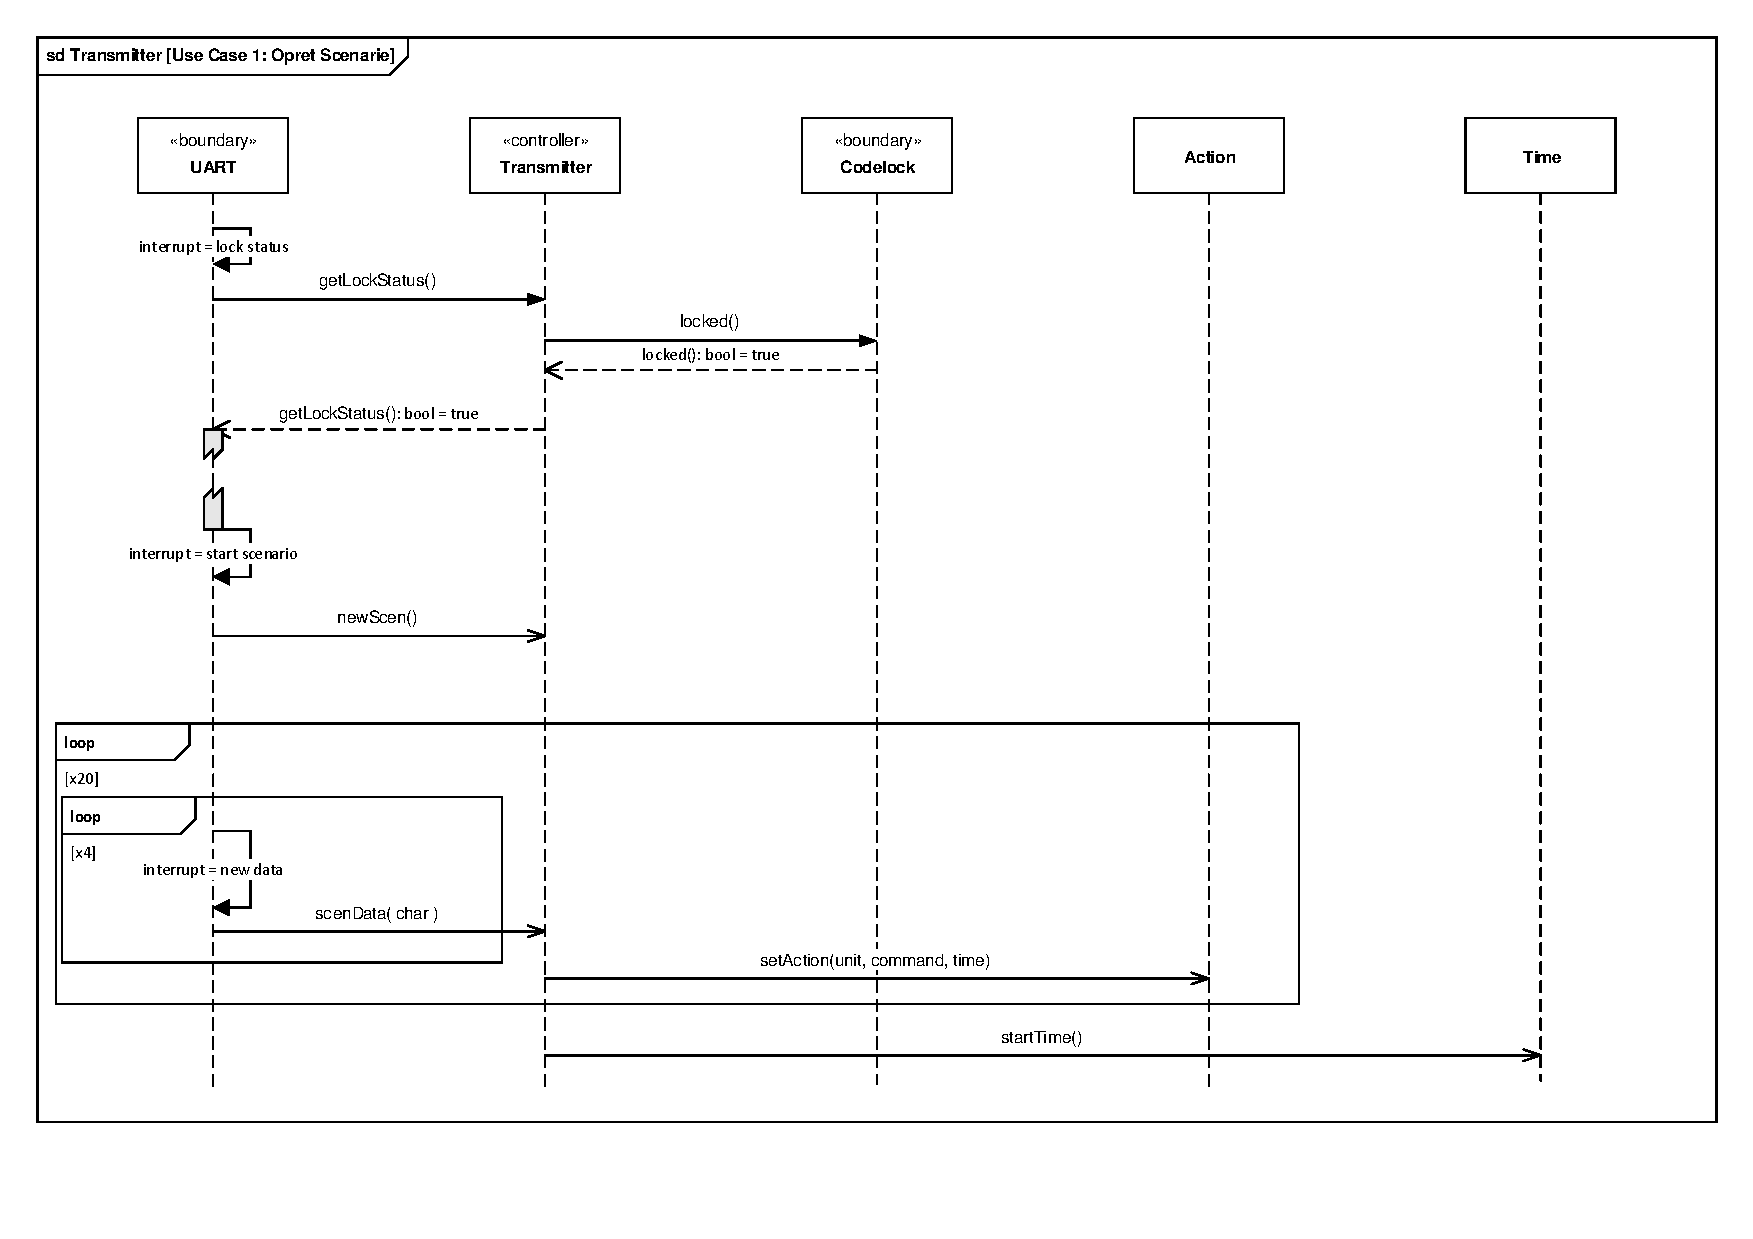
\includegraphics[height={\textwidth - 3.2 cm},trim=18 50 17 17, clip=true]{Systemarkitektur/Diagrammer/Transmitter_UC1_Sekvens.pdf}%}
	\caption{Sekvensdiagram for transmitter [Use Case 1: Opret Scenarie]}
	\label{fig:Trans_UC1Sek}
\end{figure}
\end{landscape}

\clearpage
\subsection{Sekvensdiagram for Transmitter [Use Case 3: Stop Scenarie]}
Diagrammet viser sekvenser for transmitteren ved gennemgang af hovedscenariet i UC3.
\begin{figure}[h]
	\centering
	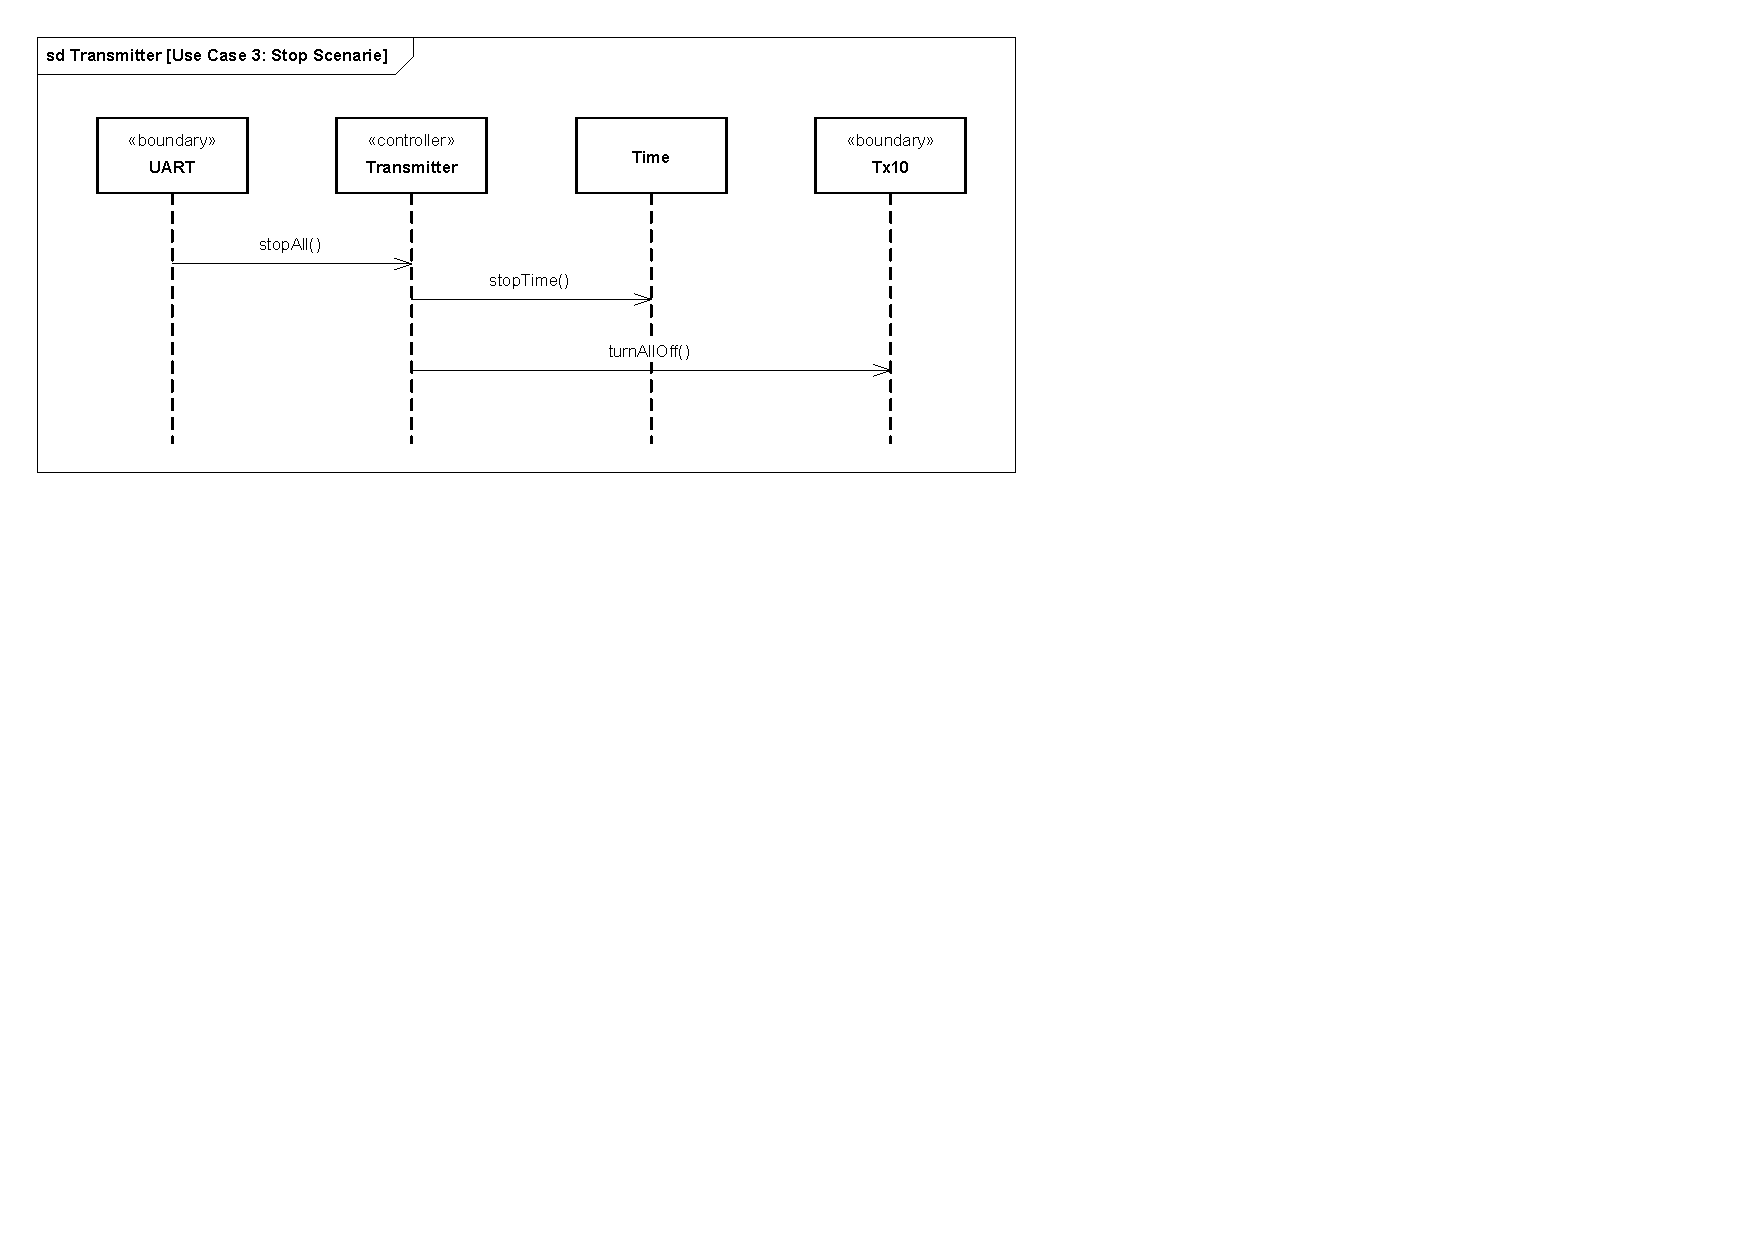
\includegraphics[width=\textwidth, trim=17 365 353 18, clip=true]{Systemarkitektur/Diagrammer/Transmitter_UC3_Sekvens.pdf}
	\caption{Sekvensdiagram for transmitter [Use Case 3: Stop Scenarie]}
	\label{fig:Trans_UC3Sek}
\end{figure}

\clearpage

\subsection{Sekvensdiagram for Transmitter [Use Case 4: Afvikl Scenarie]}
Diagrammet viser sekvenser for transmitteren ved gennemgang af hovedscenariet i UC4.
\begin{figure}[h]
	\centering 
	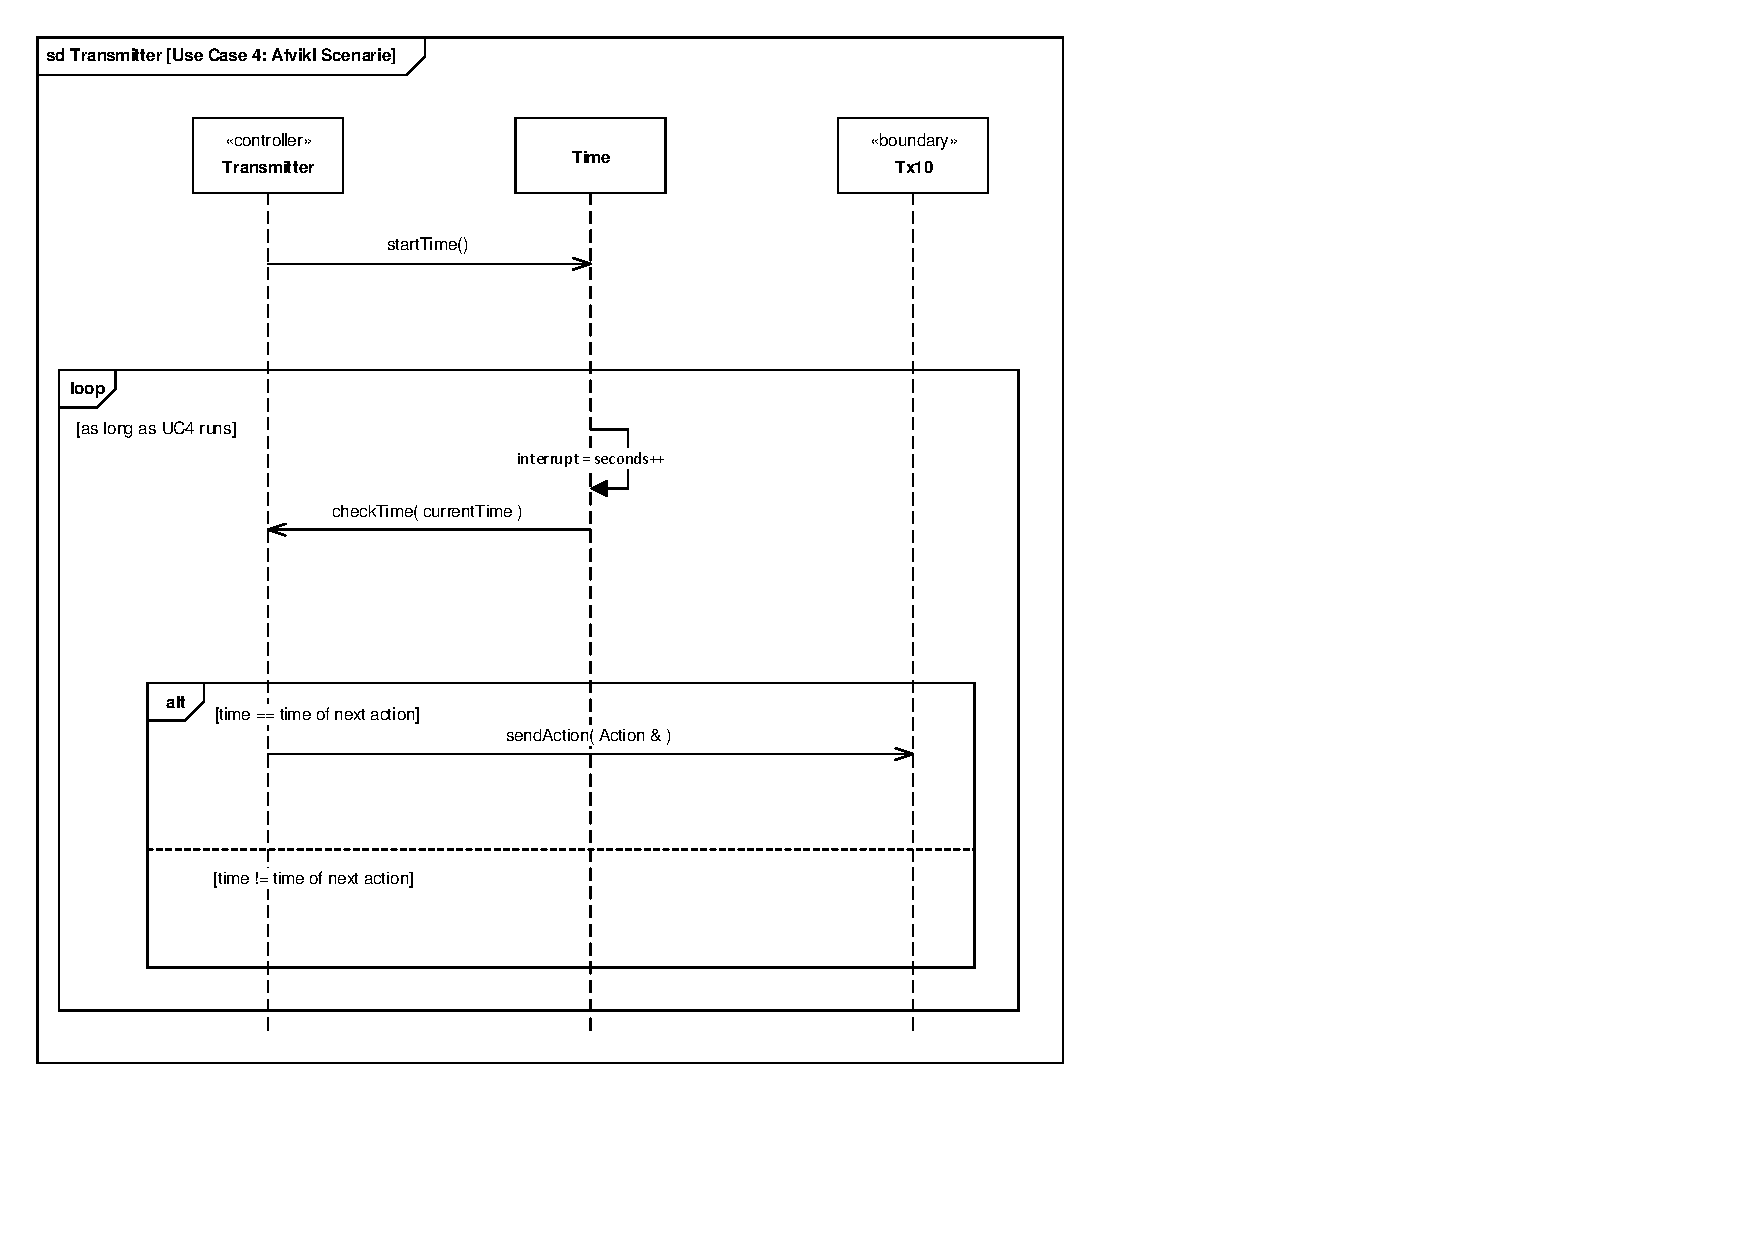
\includegraphics[width={\textwidth},trim=17 75 330 17, clip=true]{Systemarkitektur/Diagrammer/Transmitter_UC4_Sekvens.pdf}
	\caption{Sekvensdiagram for transmitter [Use Case 4: Afvikl Scenarie]}
	\label{fig:Trans_UC4Sek}
\end{figure}

\clearpage

\begin{landscape}
\subsection{Klassediagram for Transmitter}
Klassediagram for transmitter.
\begin{figure}[h]
	\centering 
	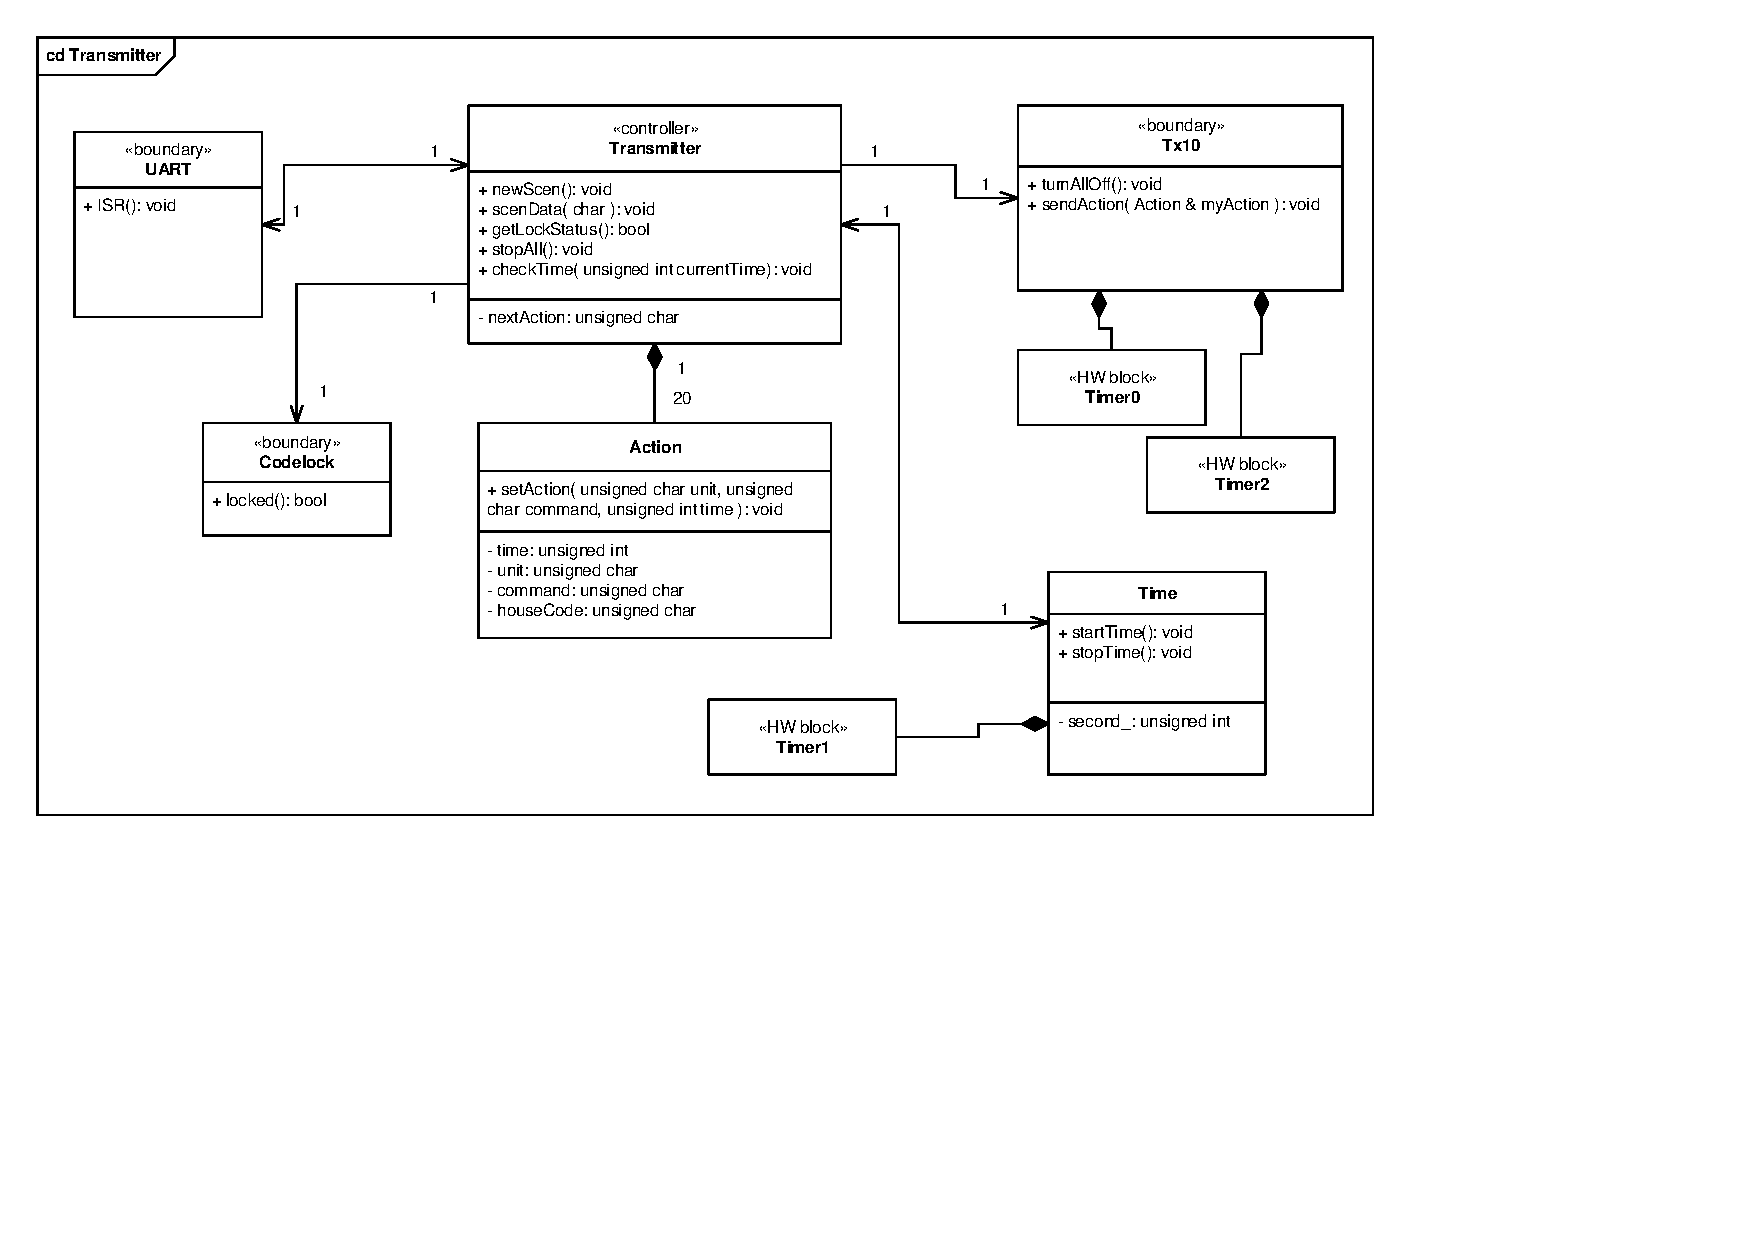
\includegraphics[height={\textwidth - 3.5 cm},trim=17 195 180 18, clip=true]{Systemarkitektur/Diagrammer/Transmitter_Klassediagram.pdf}
	\caption{Klassediagram for transmitter}
	\label{fig:Trans_Klasse}
\end{figure}
\end{landscape}

\clearpage

\subsection{Sekvensdiagram for Receiver [Use Case 4: Afvikl Scenarie]}
Diagrammet viser sekvenser for receiveren ved gennemgang af hovedscenariet i UC4. Rx10 bufferen kan forklares ved en buffer, der gemmer de seneste 8 nulgennemgange fra X.10. \emph{specified method call} er et kald af en af metoderne i klassen \texttt{Lampe}, se Figur \ref{fig:Rec_klasse}.

\begin{figure}[h]
	\centering 
	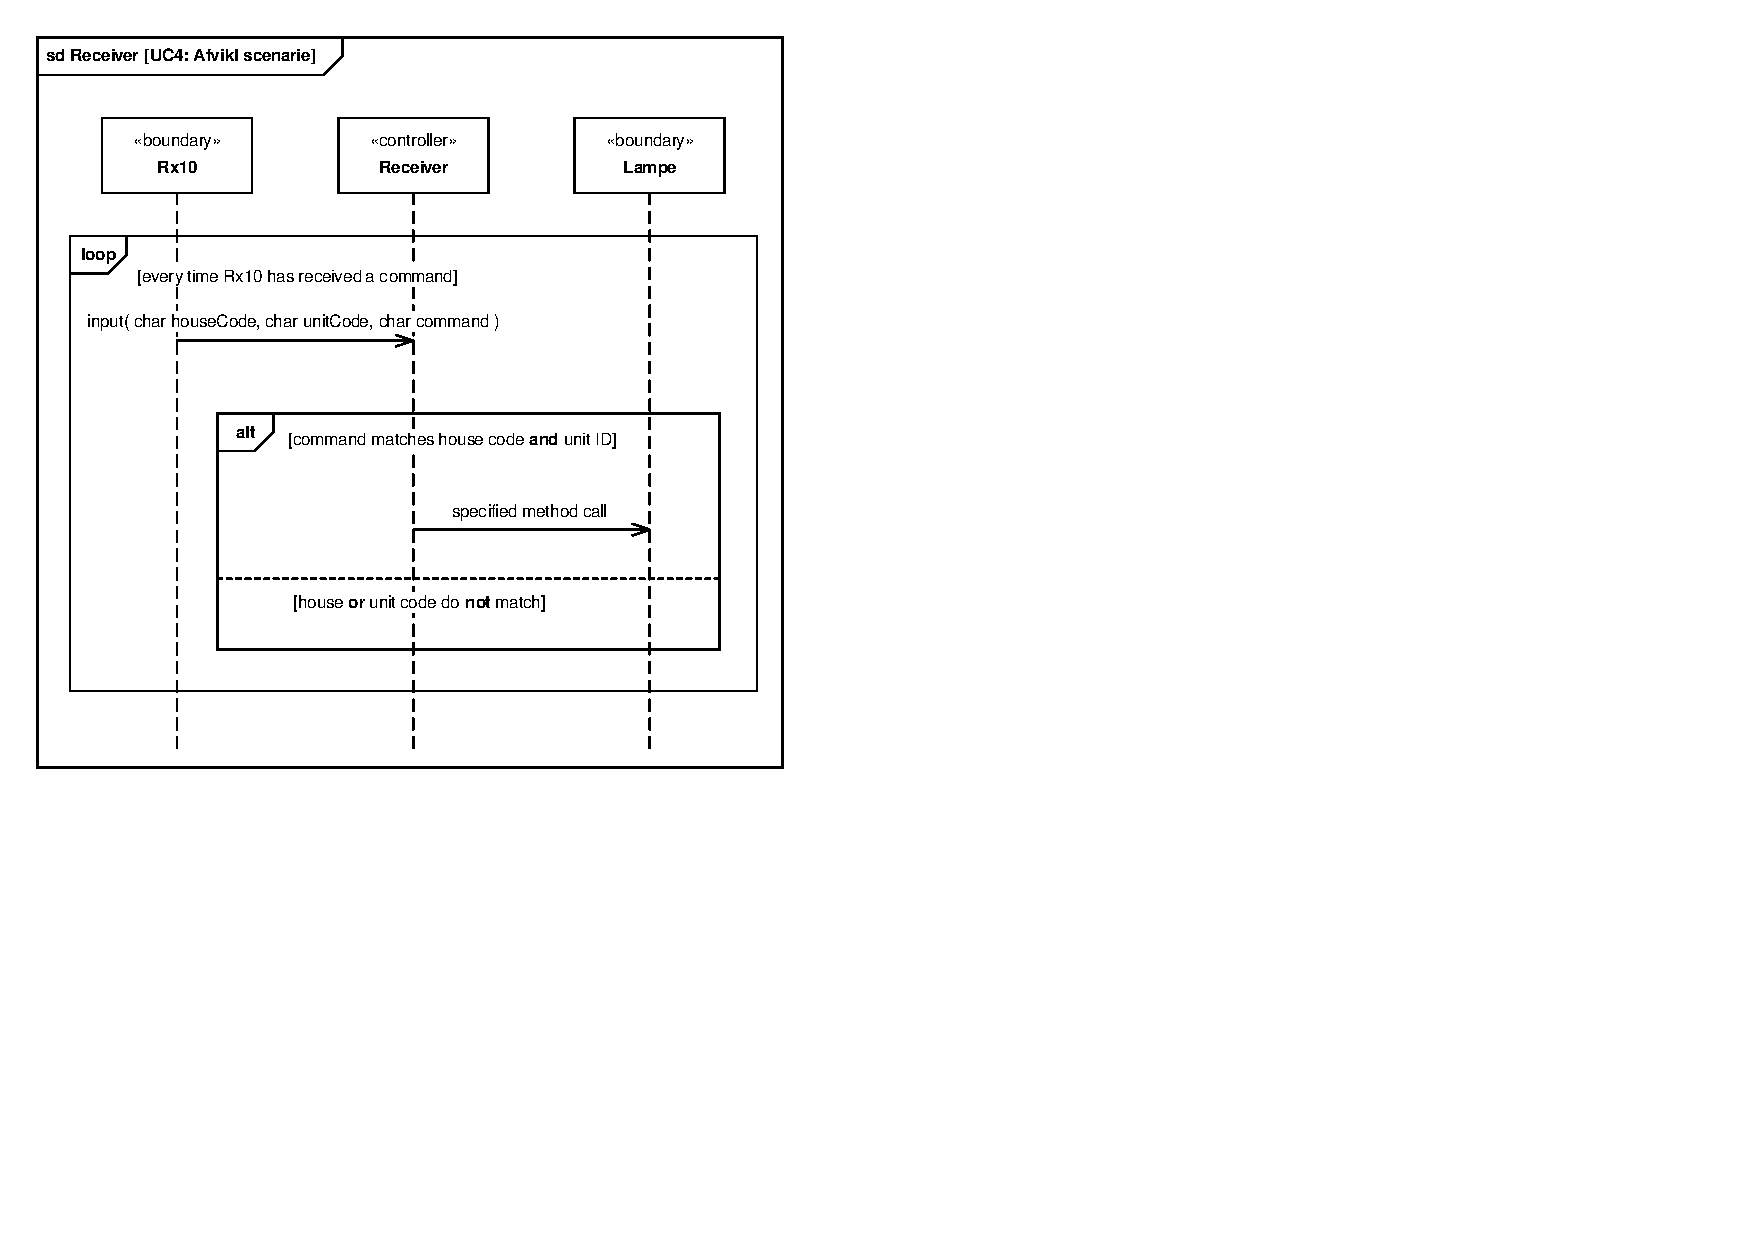
\includegraphics[scale=1,trim=17 225 465 17, clip=true]{Systemarkitektur/Diagrammer/Receiver_UC4_Sekvens.pdf}
	\caption{Sekvensdiagram for transmitter [Use Case 4: Afvikl Scenarie]}
	\label{fig:Rec_UC3Sek}
\end{figure}

\clearpage

\subsection{Klassediagram for Receiver}
Diagrammet viser klassediagram for den software, der ligger på receiveren med controller- og boundary klasse(r). Boundary klassen Rx10 har til formål at fortolke information fra hardware receiver blokken og gør det tilgængeligt for controller klassen Receiver. Boundary klassen Lampe har til formål at formidle kommunikation mellem controller klassen Receiver og hardware receiver blokken.
\begin{figure}[h]
	\centering 
	\includegraphics[width=\textwidth, trim=17 385 324 17, clip=true]{Systemarkitektur/Diagrammer/Receiver_Klassediagram.pdf}
	\caption{Klasse diagram for receiver}
	\label{fig:Rec_klasse}
\end{figure}

\clearpage